\documentclass[aps,prl,reprint]{revtex4-1}
\usepackage{blindtext}
\usepackage{ mathrsfs }
\usepackage{cleveref}
\usepackage{amsmath}
%\usepackage[justification=centering]{caption}
\usepackage{graphics,setspace,enumitem,graphicx,textpos}
\begin{document}
\bibliographystyle{plain}
\title{	Analysis of Matter and Dark Energy Content of the Universe via MCMC fitting of Type Ia Supernova Data}
\author{Delilah Gates}
\email{dgates@g.harvard.edu}
\author{Ann Wang}
\email{annwang@g.harvard.edu}
\affiliation{Harvard University}
%\begin{spacing}{1.2}
\begin{abstract}
%Something about cosmology abstract TBA
\end{abstract}
\maketitle
\section{I. Introduction}
One compelling question in cosmology research today is why the energy budget of the universe is dominated by dark energy, or a cosmological constant. Since the observation of Type Ia supernovae showed that the universe was expanding at an accelerated rate, dark energy research has been an active area of study \cite{riess_sn}. Recently, a study by J.T. Nielson et al. \cite{shocker} claimed, analyzing a larger set of supernovae data, that there was little evidence for an accelerated rate of expansion. We reanalyze the same data set and present our findings here.
\section{II. Background}
To compare results, we use data from the Joint Lightcurve Analysis (JLA) catalog \cite{sdss}, which uses the Spectral Adaptive Lightcurve Template 2 (SALT2) approach to characterize Type Ia Supernovae \cite{salt2}. This combines the recent SDSS-II survey along with several past surveys from other experiments \cite{sdss}. There are several versions of the covariance matrix for the distance modulus; we use the covmat\_v6 version along with the corresponding code to convert the covariance data from FITS format \cite{fits} to a matrix format given $\alpha$, $\beta$ (see later $\mu$ equation), which was provided at http://supernovae.in2p3.fr/sdss\_snls\_jla/ReadMe.html. 
\par The data provides us with several characteristic values for every SN Ia: the heliocentric redshift $z_{hel}$, the CMB frame redshift $z_{CMB}$, the apparent magnitude $m_B$, the shape parameter from SALT2, $x_1$, the color correction $c$, and the host stellar mass $M_{stellar}$ \cite{sdss}. Using these parameters, we can define a distant modulus which can be compared to a value expected by a certain cosmological model. This distance modulus is given by \cite{sdss}: 
\begin{equation}
\mu = m_B - M + \alpha x_1 - \beta c
\end{equation}
The M, or absolute magnitude, is dependent on the host galaxy, so we follow the prescription in \cite{sdss}, where if $M_{stellar} < 10^{10} M_{\odot}$, then $M_B = M_B'$, otherwise, $M_B = M_B' + \Delta_M$. 

For comparison, using the density parameters ($\Omega_m$, $\Omega_{r}$, $\Omega_{\Lambda}$) and curvature ($\Omega_k$) of a comological model one can calculate the distance modulous of an object at a certain redshift as follows:  
$$E(z)=\sqrt{\Omega_{r}(1+z)^4 + \Omega_m(1+z)^3 + \Omega_k(1+z)^2 + \Omega_{\Lambda}} $$
$$d_L(z)=\frac{c}{H_0} {\int_0}^z \frac{dz'}{E(z')} $$
$$\mu = 25 + 5\;\text{log}_{10} \left( \frac{d_L(z)}{\text{Mpc}} \right) $$
 
dfd
\section{III. Methods}
We perform a likelihood analysis using MCMC methods. Our code can be found online at https://github.com/deagates/CosmologySNProject.
\par We will adopt the likelihood function described in \cite{sdss}, which is defined to be $$\mathscr{L} = \text{exp}(-\frac{\chi^2}{2}) $$ where$$\chi^2 = (\hat{\mu}-\mu_\text{model})^\dagger C^{-1} (\hat{\mu}-\mu_\text{model}),$$  with C as the covariance matrix, and $\hat{\mu}$ and $\mu_\text{model}$ are calculated using (1) and (2) respectively . For simplicity and comparability with J.T. Nielson et al., we take $\Omega_r$ the radiation density parameter of the universe to be 0, further justified by the fact that the measured radiation density parameter of today is very small, and we assume the universe is flat ($\Omega_k = 0$). This leaves us with the constraint that $\Omega_m + \Omega_{\Lambda} = 1 $. We have five model parameters ($\Omega_m$, $\alpha$, $\beta$, $M'_B$, and $\Delta_M$) that our MCMC varies to try to maximize the likelihood.
\par The covariance matrix, provided at the aforementioned database, is composed of several errors. Equation (11) of \cite{sdss} describes the covariance matrix as: \begin{math}  \newline \newline  \indent \indent \indent \indent  C_\eta = C_{\text{stat}} + (C_{\text{cal}} + C_{\text{model}} + C_{\text{bias}} \newline
\indent \indent  + C_{\text{host}} + C_{\text{dust}})_{\text{reevaluated}} + (C_{\text{pecvel}}+C_{\text{nonIa}})_{\text{C11}}.\end{math}
\newline \par Included in this matrix are: the statistical uncertainties encompass the light-curve fit uncertainties, the photometric calibration uncertainties, uncertainties associated with the light-curve model, uncertainties associated with selection biases from the surveys, the uncertainties of the host masses, an uncertainty to limit sensitivity to Milky Way dust extinction, and two uncertainties taken from the compilation of all of the supernova data not from SDSS (i.e. SNLS, HST, etc.) from Conley et al. \cite{c11}. This is then combined to calculate the covariance matrix of the distance modulus, which is defined in eq. 13 of \cite{sdss} as follows:
$$C = A C_\eta A^\dagger + \text{diag}(\frac{5\sigma_z}{z \text{log} 10})^2 + \text{diag}(\sigma_\text{lens}^2) + \text{diag}(\sigma_{\text{coh}}^2). $$
This combines more uncertainties on the redshift, additional effects from gravitational lensing, and a catch-all term for other uncertainties on the magnitudes. We use the final $C$ matrix in the calculation of our likelihoods. 
\par We ran our MCMC analyzer for INSERT NITER iterations, each with 20,000 steps. The prior distributions on the five fit parameters were all flat, with bounds as follows:
\begin{center}
\begin{tabular}{ |c|c|c| } 
 \hline
 \textbf{Parameter} & \textbf{Upper Bound} & \textbf{Lower Bound} \\ 
 $\Omega_M$ & 0 & 1 \\ 
 $\alpha$ & -1 & 4 \\ 
 $\beta$ & 1 & 6 \\ 
 $M'_B$ & -21 & -17 \\ 
$\Delta_M$ & -2 & 1 \\ 
 \hline
\end{tabular}
\end{center}
\par After the initial random draw of the parameter, the next iterative parameter value was picked using a random draw from a normal distribution centered around the current parameter value with a $\sigma$ of 0.5 for $\Omega_M$ and a $\sigma$ of 0.8 for the nuisance parameters. These values were hand-tuned by running several test runs and looking at the trace plots, shown in \cref{fig:alpha,fig:om,fig:mp,fig:dm,fig:beta}. 
\begin{figure}
 %\centering
 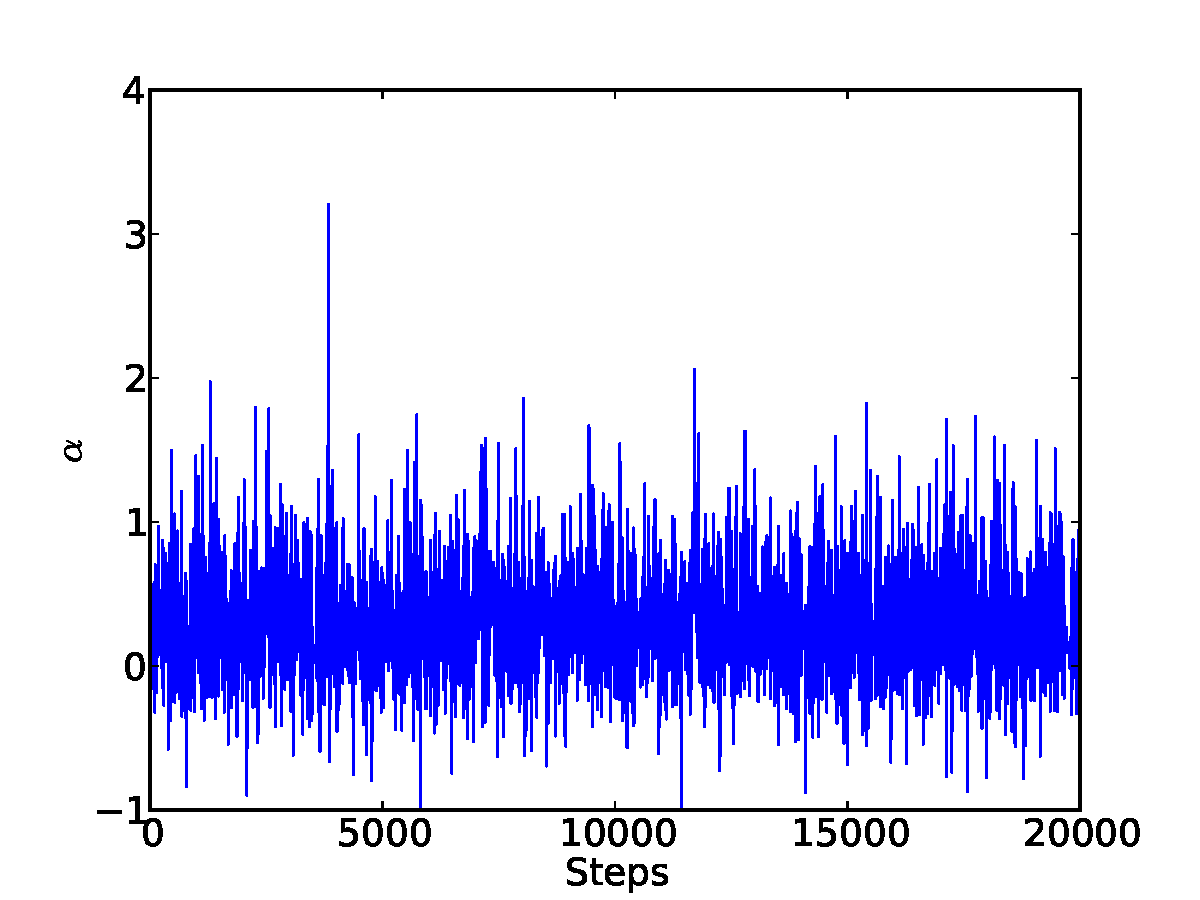
\includegraphics[width=0.5\textwidth]{../plots/alpha.pdf}
\caption{\label{fig:alpha}An example of a $\alpha$ trace plot for one of the MCMC iterations.}
\end{figure}
\begin{figure}
 %\centering
 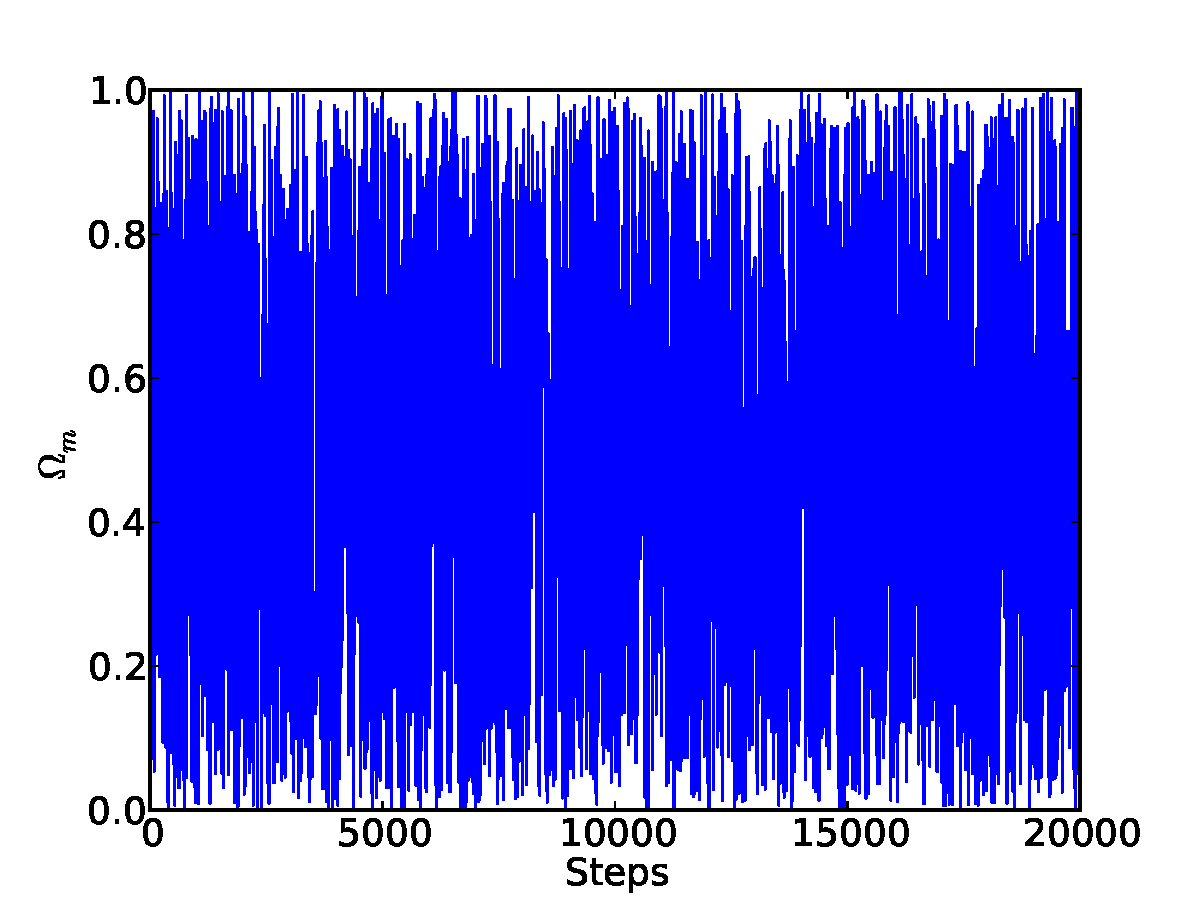
\includegraphics[width=0.5\textwidth]{../plots/om.pdf}
\caption{\label{fig:om}An example of a $\Omega_M$ trace plot for one of the MCMC iterations.}
\end{figure}
\begin{figure}
 %\centering
 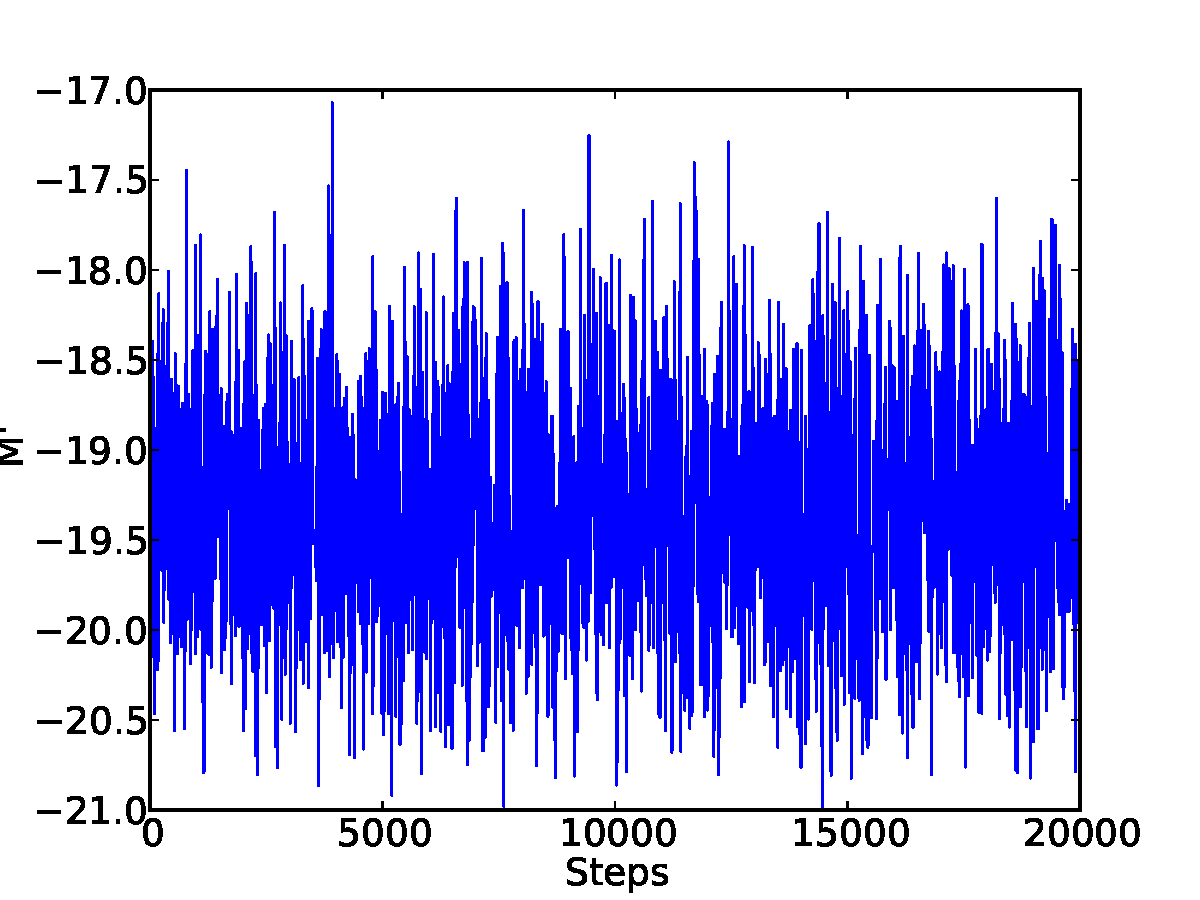
\includegraphics[width=0.5\textwidth]{../plots/Mp.pdf}
\caption{\label{fig:mp}An example of a  $M'_B$ trace plot for one of the MCMC iterations.}
\end{figure}
\begin{figure}
 %\centering
 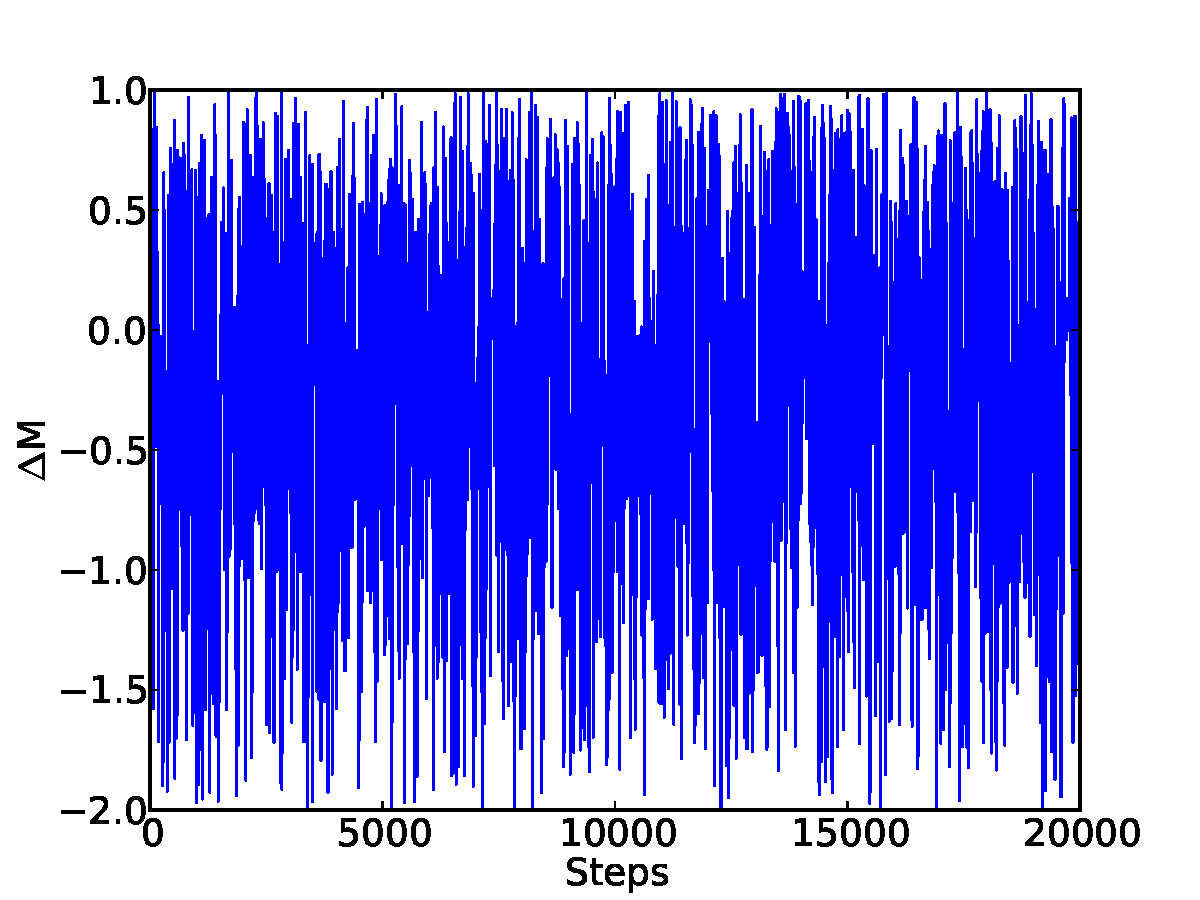
\includegraphics[width=0.5\textwidth]{../plots/dM.pdf}
\caption{\label{fig:dm}An example of a  $\Delta_M$ trace plot for one of the MCMC iterations.}
\end{figure}
\begin{figure}
 %\centering
 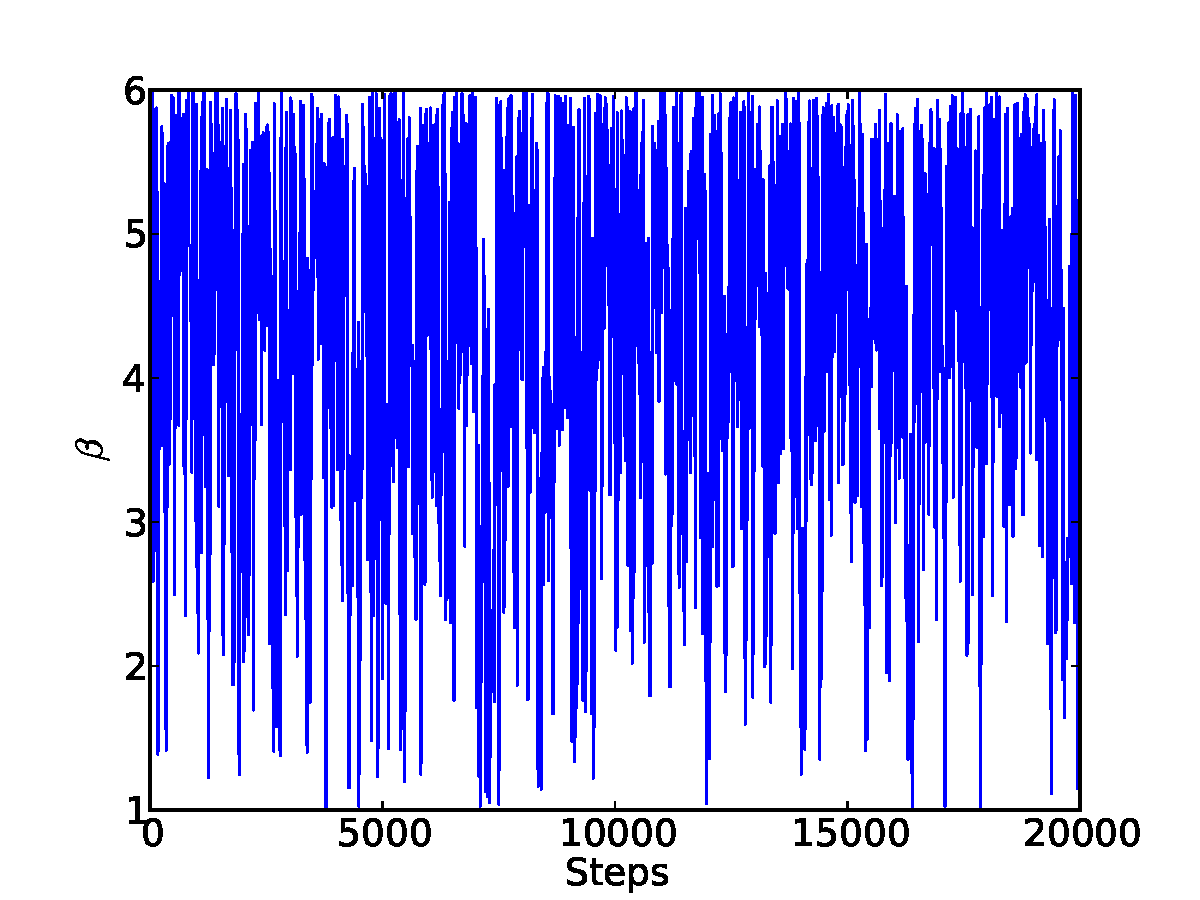
\includegraphics[width=0.5\textwidth]{../plots/beta.pdf}
\caption{\label{fig:beta}An example of a  $\beta$ trace plot for one of the MCMC iterations.}
\end{figure}
\begin{figure}
 %\centering
 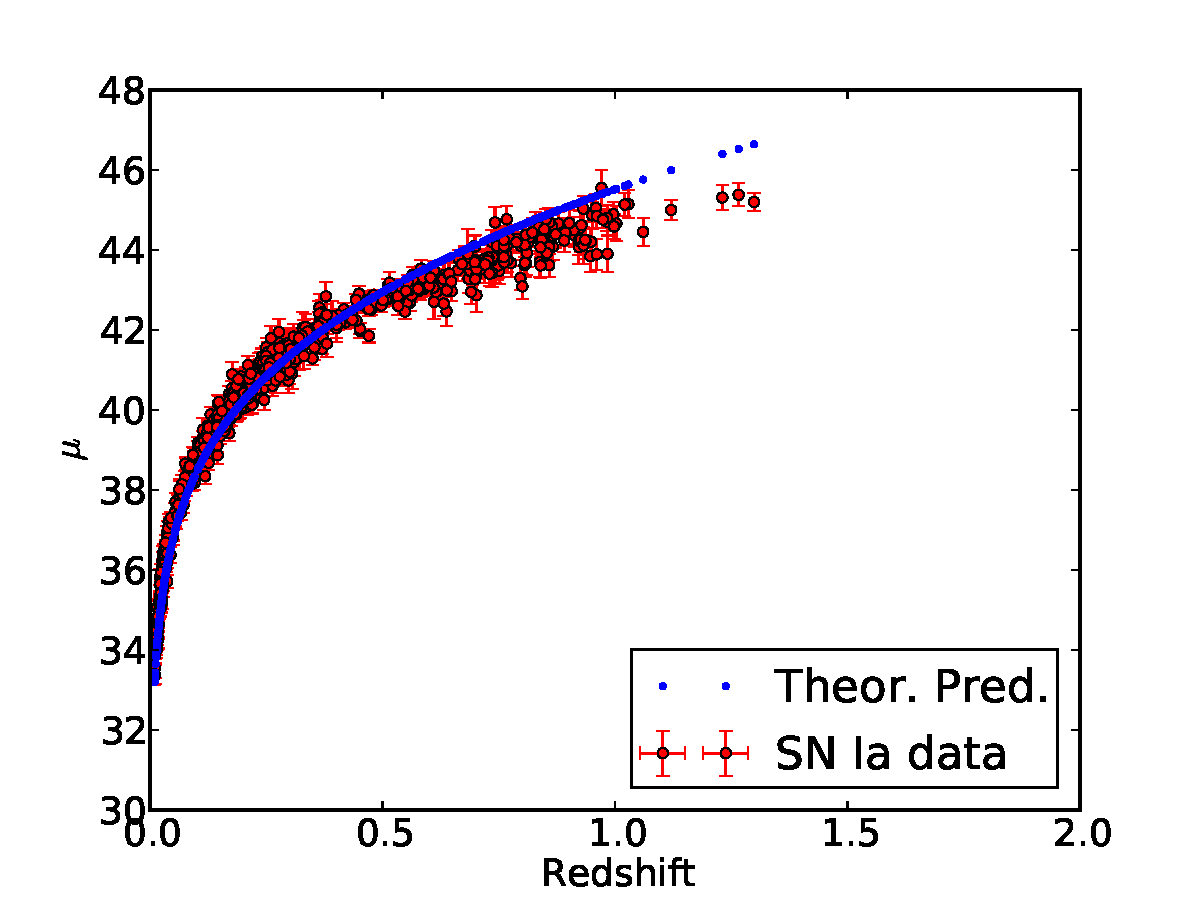
\includegraphics[width=0.5\textwidth]{../plots/mu.pdf}
\caption{\label{fig:mu}The distribution of distance modulii versus redshift for the SN Ia points used in the analysis from the JLA catalog. The $\mu_\text{model}$ distribution predicted by our best-fit value of $\Omega_l$, $\Omega_m$ is overlaid in blue.}
\end{figure}
\section{IV. Analysis} 
\section{V. Discussion}
Our approach follows the steps of \cite{sdss}, using the same likelihood function and fit parameters. In future studies, to make a direct comparison with J.T. Nielson et al., our approach can be expanded to adopt their likelihood function. 
They employ an alternative likelihood function, which they define as \begin{align*}\mathscr{L} = |2\pi(C+A^T \Sigma_l A)|^{-1/2}\; \\
\times \text{Exp}[-(\hat{Z}-Y_0A)(C+A^T\Sigma_lA)^{-1}(\hat{Z}-Y_0A)^T/2],\end{align*} where $\Sigma_l = \text{diag}[\sigma_{M_0}^2,\sigma_{X_{1,0}}^2,\sigma_{C_0}^2,...],$ $A = ,$ $\hat{Z} = [\hat{m}_{B1}-\mu_1, \hat{x}_{11},\hat{c}_1,..]$, and $Y_0 = [M_0,x_{1,0},c_0,....]$. 
\par To make a more accurate comparison, this likelihood function should be implemented and compared directly to the $\chi^2$ likelihood function. Then, the authors' reported effect of the alternative likelihood measure could be accurately evaluated while keeping all of the other conditions (such as the host stellar mass handling) the same. 


 
\bibliographystyle{apsrev4-1} % Tell bibtex which bibliography style to use
\bibliography{cosmo_bib} 
\end{document}
